% !TEX program = pdflatex
% !TEX options = -synctex=1 -interaction=nonstopmode -file-line-error -shell-escape "%DOC%"
\documentclass{beamer}
\usepackage{hyperref}
\usepackage{graphicx,url}
\usepackage[brazil]{babel}   
\usepackage[utf8]{inputenc}
\usepackage{pgf,tikz}
\usepackage{soul}
\usepackage{adjustbox}
\usepackage{mathrsfs}
\usepackage{listings}
\usepackage{minted}
\usetikzlibrary{calc}
\usetikzlibrary{arrows}
\batchmode
\usepackage{amsmath,amssymb,enumerate,epsfig,bbm,calc,color,ifthen,capt-of}
\usetheme{Berlin}
%-------------------------Titulo/Autores/Orientador------------------------------------------------
\title[Tree and Recursion]{
  Tree and Recursion
}
\subtitle {Monash ICPC workshop}
\date{}
\author[Shizhe Zhao]{
  Shizhe Zhao
}

\pgfdeclareimage[height=1.5cm]{monash-logo}{icpc.pdf}
\logo{\pgfuseimage{monash-logo}\hspace*{0.5cm}}

% -----------------------------------------------------------------------------
\begin{document}
% -----------------------------------------------------------------------------

%---Summary---------------------------------------------------------
\frame{\titlepage}

\begin{frame}{About the workshop}
  What's not?
  \begin{itemize}
    \item Not a revising of lectures 
    \item No spoon-feeding 
  \end{itemize}

  What's it?
  \begin{itemize}
    \item Beyond your algo-units: extensions, application ...
    \item Filling up the gap between knowledge and practice.
    \item Develop your problem-solving skill
  \end{itemize}
\end{frame}

\begin{frame}
  \frametitle{Intro: Tree structure in CS}
Search space
\begin{figure}[]
  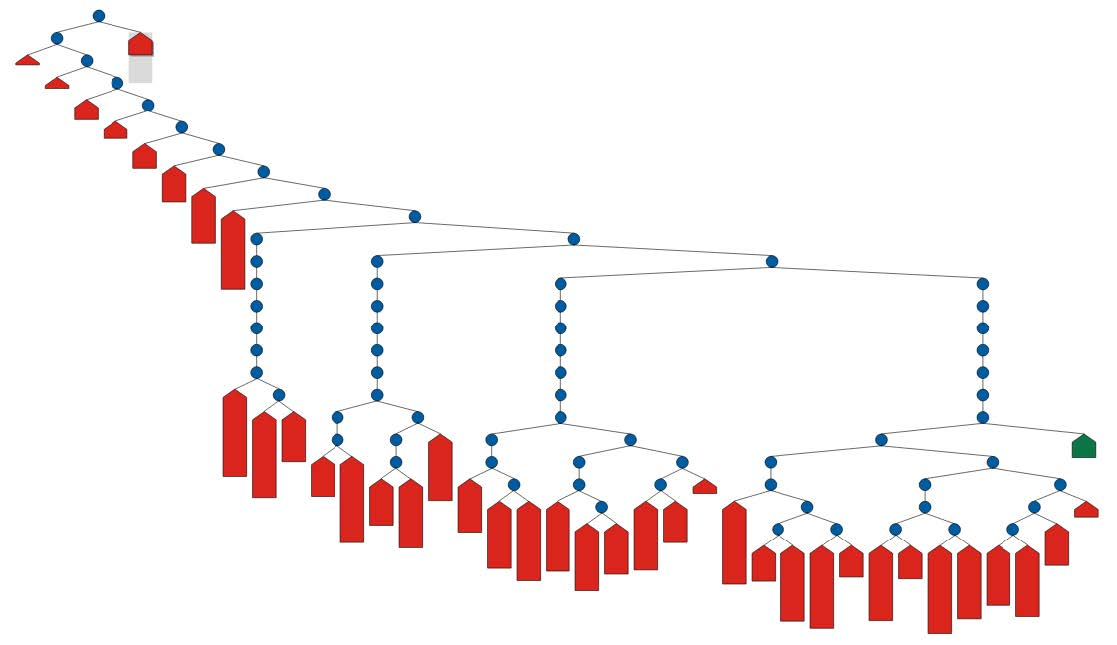
\includegraphics[width=.7\textwidth]{./figs/search-tree.jpg} 
\end{figure}
 \tiny {Search space of a MiniZinc solver}
\end{frame}

\begin{frame}[fragile]
  \frametitle{Intro: Tree structure in CS}
Syntax
\begin{minted}[frame=lines, fontsize=\footnotesize]{sql}
 SELECT id, name FROM t_user WHERE status = 'ACTIVE' AND age > 18
\end{minted}
\begin{figure}[]
  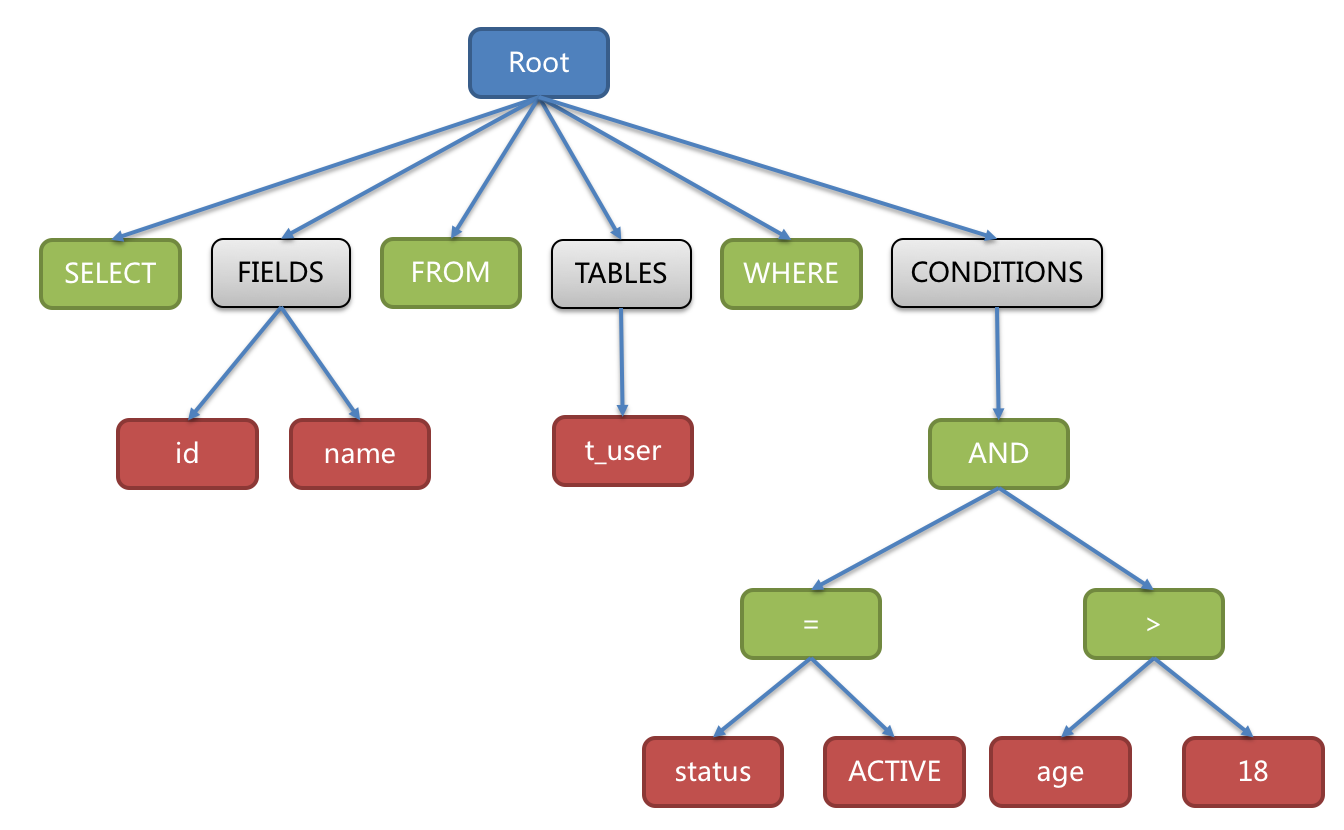
\includegraphics[width=.65\textwidth]{./figs/sql_ast.png}
\end{figure}
\end{frame}

\begin{frame}
  \frametitle{Intro: Tree structure in CS}
The most common recursion structure, classic examples:
\begin{itemize}
  \item Tree traversal (Pre/In/Post, DFS)
  \item Dynamic Programming on tree
\end{itemize}
\end{frame}

\begin{frame}[fragile]
  \frametitle{Tree traversals - quick review}
\begin{minipage}{.5\textwidth}
\begin{minted}[fontsize=\footnotesize]{python}
# Binary tree
def preorder(root):
  if root:
    visit(root)
    preorder(root.left)
    preorder(root.right)

def inorder(root):
  if root:
    inorder(root.left)
    visit(root)
    inorder(root.right)
\end{minted}
\end{minipage}%
\begin{minipage}{.5\textwidth}
\vspace{-2mm}
\begin{minted}[fontsize=\footnotesize]{python}
def postorder(root):
  if root:
    postorder(root.left)
    postorder(root.right)
    visit(root)

# Generic tree
def dfs(root):
  visit(root)
  for c in root.children:
    dfs(c)
  leave(root)
\end{minted}  
\end{minipage}
\end{frame}

\begin{frame}
  \frametitle{Applications of traversals}
\begin{itemize}
  \item <1-> Expression tree: pre/ dfs order
  \item <2-> Binary search tree: in order
  \item <3-> Deleting the tree: post order
  \item <4-> Map a tree to a vector. 
  \begin{itemize}
    \only<5> {\item Then you can feed the vector to a neural network, magic!}
    \only<6-> {\item \st{Then you can feed the vector to a neural network, magic!}}
    \item<7-> Then you can represent a subtree by "slicing", magic!
    \item<8-> LCA (Lowest Common Ancestor).
  \end{itemize}
\end{itemize}

\only<9-> {Hope we can cover these topics in the future.}
\end{frame}

\begin{frame}
  \frametitle{Example: Tree Visualisation}
\vspace{-5mm}
\begin{figure}[]
  \centering
  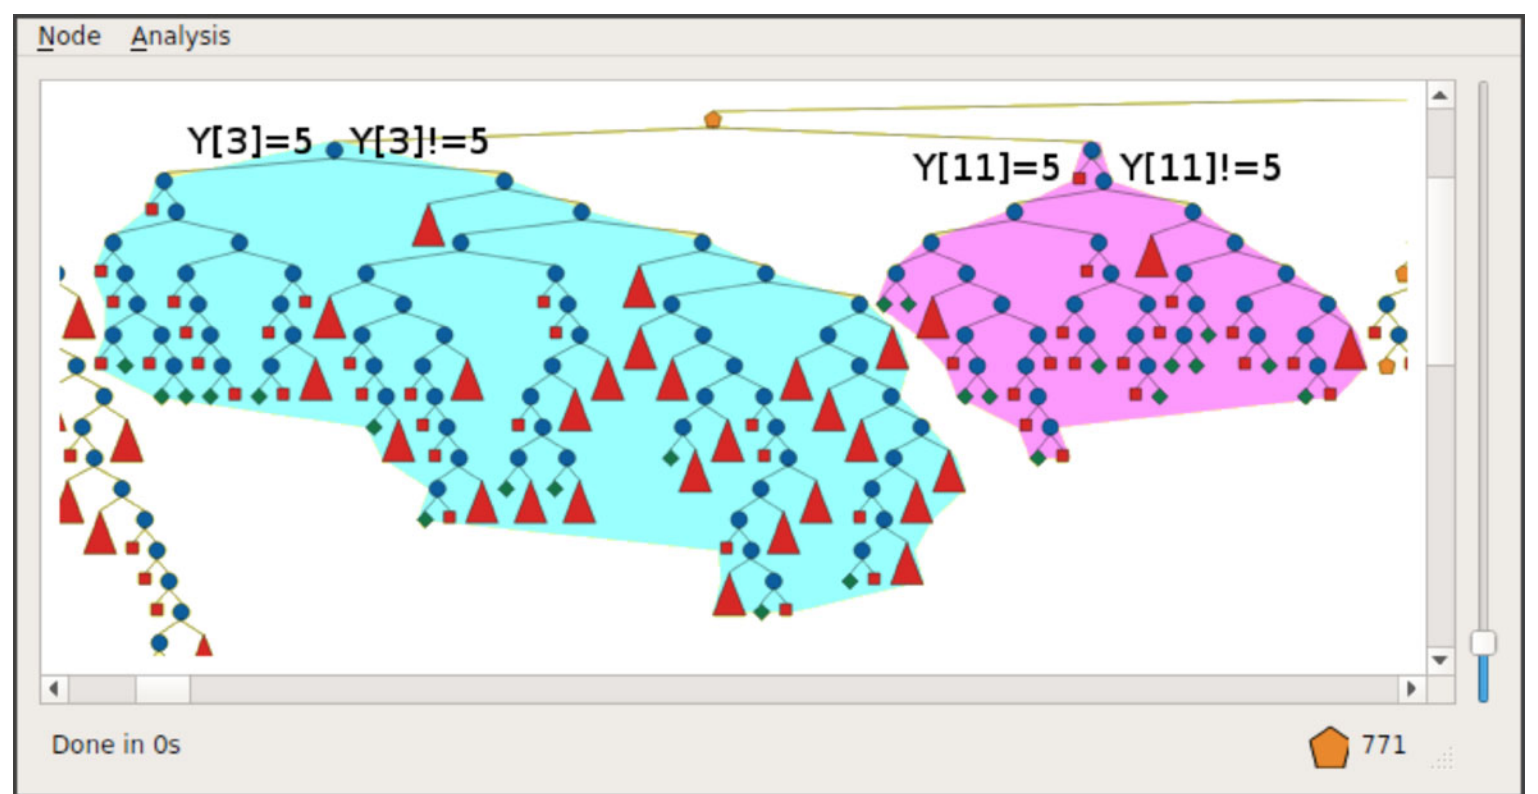
\includegraphics[width=.9\textwidth]{figs/visual-tree.png} 
\end{figure}
\small{
Visualize a tree with more than 10M nodes.

Scroll left/right/up/down.
}
\end{frame}

\begin{frame}
  \frametitle{Example: Tree Visualisation}
\begin{itemize}
  \item solution-1: \texttt{\small render(tree)} and only show visible part \footnote{\url{https://researchmgt.monash.edu/ws/portalfiles/portal/257776846/3566886_oa.pdf}}
  \begin{itemize}
    \item rendering: 15s
    \item scrolling delay: 200ms
  \end{itemize}

  \item solution-2: \texttt{\small render(leftMostId, rightMostId)} and show \footnote{\url{https://github.com/eggeek/cp-profiler}}
  \begin{itemize}
    \item rendering: 200ms 
    \item scrolling delay: 20ms
  \end{itemize}
\end{itemize}
\vspace{5mm}
\large {Data structure is important!}
\end{frame}

\begin{frame}
  \frametitle{Example 2: \href{https://vjudge.net/contest/364479\#problem/A}{Company Party}}

Brief:
\begin{itemize}
  \item There are $n$ employees, each one has 0 or 1 direct leader - forest structure
  \item Employees can not in a party group that contains their ancestor
  \item What's the minimum number of group?
\end{itemize}

\end{frame}

\begin{frame}[fragile]
  \frametitle{Example 2: \href{https://vjudge.net/contest/364479\#problem/A}{Company Party}}
\begin{minted}[linenos=true, frame=lines, fontsize=\footnotesize]{python}
def dfs(i):
  if fa[i] == -1:
    return 1
  return dfs(fa[i]) + 1

n = int(input())
fa = [0] * (n+1)
for i in range(1, n+1):
  fa[i] = int(input())
res = max([dfs(i) for i in range(1, n+1)]) 
print (res)
\end{minted}

Bottom to top - $O(n^2)$.
\end{frame}

\begin{frame}[fragile]
  \frametitle{Example 2: \href{https://vjudge.net/contest/364479\#problem/A}{Company Party}}
\begin{minted}[linenos=true, frame=lines, fontsize=\scriptsize]{python}
def dfs(i, dep):
	if fa[i] == -1:
		return 1
	if dep[i] > 0:
		return dep[i]
	dep[i] = dfs(fa[i], dep) + 1
	return dep[i]

n = int(input())
fa = [0] * (n+1)
for i in range(1, n+1):
	fa[i] = int(input())
dep = [0] * (n+1)
res = max([dfs(i, dep) for i in range(1, n+1)]) 
print (res))
\end{minted}

With memorization - $O(n)$ .
\end{frame}

\begin{frame}[fragile]
  \frametitle{Common Patterns}
\begin{minted}[linenos=true, frame=lines, fontsize=\scriptsize]{python}
import sys
# you may need to reset stack limit, 
# usually default is 1000
sys.setrecursionlimit(...)

# Undirected
def dfs(pre, node, graph):
  for i in graph.neighbors:
    if i != pre:
      dfs(node, i, graph)
\end{minted}

Line $9$ is important!

\end{frame}

\begin{frame}
  \frametitle{Coding time!}
  \begin{itemize}
    \item \url{https://vjudge.net/contest/364479}
  \end{itemize}
\end{frame}
% -----------------------------------------------------------------------------
\end{document}
%-----------------------------------------------
